\documentclass[12pt,letterpaper]{article}
\usepackage[utf8]{inputenc}
\usepackage[spanish]{babel}
\usepackage{graphicx}
\usepackage[left=2cm,right=2cm,top=2cm,bottom=2cm]{geometry}
\usepackage{graphicx} % figuras
% \usepackage{subfigure} % subfiguras
\usepackage{float} % para usar [H]
\usepackage{amsmath}
%\usepackage{txfonts}
\usepackage{stackrel} 
\usepackage{multirow}
\usepackage{enumerate} % enumerados
\renewcommand{\labelitemi}{$-$}
\renewcommand{\labelitemii}{$\cdot$}
% \author{}
% \title{Caratula}
\begin{document}

% Fancy Header and Footer
% \usepackage{fancyhdr}
% \pagestyle{fancy}
% \cfoot{}
% \rfoot{\thepage}
%

% \usepackage[hidelinks]{hyperref} % CREA HYPERVINCULOS EN INDICE

% \author{}
\title{Caratula}

\begin{titlepage}
\begin{center}
\large{UNIVERSIDAD PRIVADA DE TACNA}\\
\vspace*{-0.025in}
\begin{figure}[htb]
\begin{center}

\includegraphics[width=7cm]{./images/logo}
\end{center}
\end{figure}
\vspace*{0.15in}
INGENIERIA DE SISTEMAS  \\

\vspace*{0.3in}
\begin{large}
\textbf{TITULO:} \\
\end{large}

\vspace*{0.1in}
\begin{Large}
\textbf{Practica de Laboratorio Nº 03: Creando un Cubo Multimensional con SQL Server
Analysis Services} \\

\end{Large}

\vspace*{0.3in}
\begin{Large}
\textbf{CURSO:} \\
\end{Large}

\vspace*{0.1in}
\begin{large}
INTELIGENCIA DE NEGOCIOS\\
\end{large}

\vspace*{0.3in}
\begin{Large}
\textbf{DOCENTE:} \\
\end{Large}

\vspace*{0.1in}
\begin{large}
 Ing. Patrick Cuadros Quiroga\\
\end{large}

\vspace*{0.4in}
\vspace*{0.1in}
\begin{large}
\textbf{Estudiante:} \\
\begin{flushleft}
José Edilberto Pastor Mendoza  \hfill	(2016055237)\\

\centering  %CENTRA UN TEXTO
\vspace*{0.9in}
\begin{large}
Tacna\\ 
\end{large}

\end{flushleft}
\end{large}
\end{center}

\end{titlepage}


\tableofcontents % INDICE
\thispagestyle{empty} % INDICE SIN NUMERO
\newpage
\setcounter{page}{1} % REINICIAR CONTADOR DE PAGINAS DESPUES DEL INDICE

%%INICIO Resumen
\section{Objetivos}
Crear un cubo Multidimensional, para lo cual se tiene que haber instalado antes el motor de Analysis
Services Multidimensional se necesita una base de datos para la creación del cubo, para lo que se
necesitaría tener restaurada la base de datos Adventure Works DW..
%%FIN Resumen

%%----------------------------------------------------------------------------------------------------------------------------------------------------------
%%INICIO Marco Teórico
\section{Procedimiento}

Abrir el SQL Server Data Tools y dirigirnos a la pestaña de Business Intelligence -> Analysis
Services. Como se creará un Modelo Multidimensional desde 0 , seleccionaremos la primera opción. En la
casilla de Name le colocamos un nombre al proyecto y a la solución:



\begin{center}
	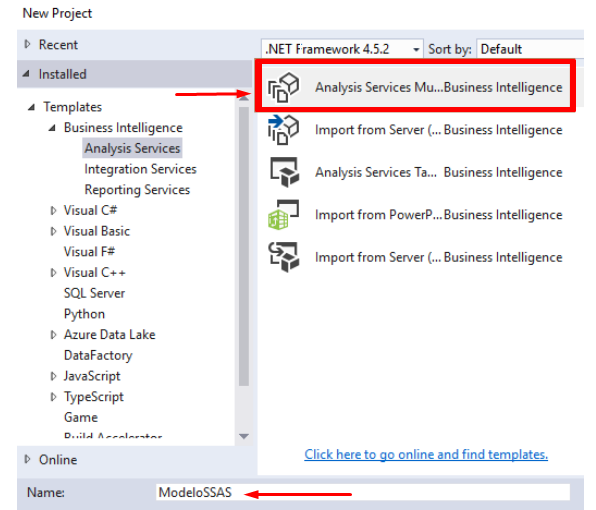
\includegraphics[width=8cm]{images/task1/img1}
\end{center}
\section{Creación de un Data Source}  
 En el Solution Explorer nos ubicamos en Data Sources y click derecho, seleccionando la opción de New
Data Source …
		

	\begin{center}
	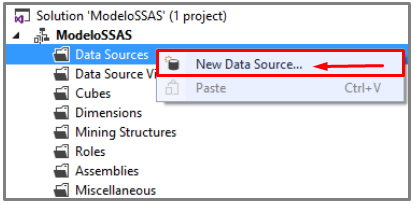
\includegraphics[width=8cm]{images/task1/img2}
	\end{center}	
Se nos abrirá una ventana de resumen. Click en Next:
	\begin{center}
	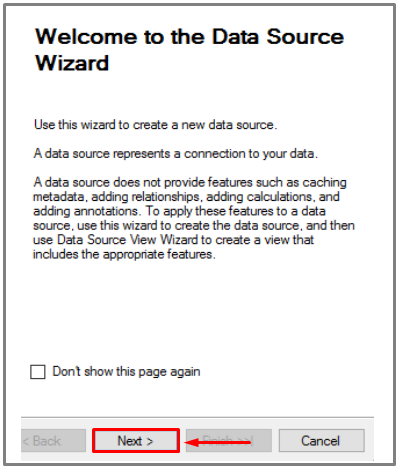
\includegraphics[width=8cm]{images/task1/img3}
	\end{center}	
Si es la primera vez que realizamos un proyecto de estos, no tendremos creadas conexiones. Click en New
para crear una nueva conexión hacia la base de datos Adventure Works DW:
	\begin{center}
	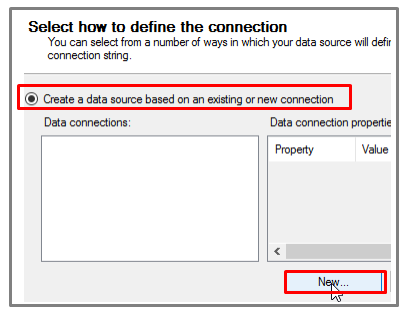
\includegraphics[width=8cm]{images/task1/img4}
    \end{center}	
Colocamos el nombre del Server donde se ubica la base de datos, en mi caso como es local coloco “.” ,
indicándole que es localhost. Ingresamos las credenciales y la base de datos Adventure Works DW 2014.
Luego Click en Ok:
	\begin{center}
	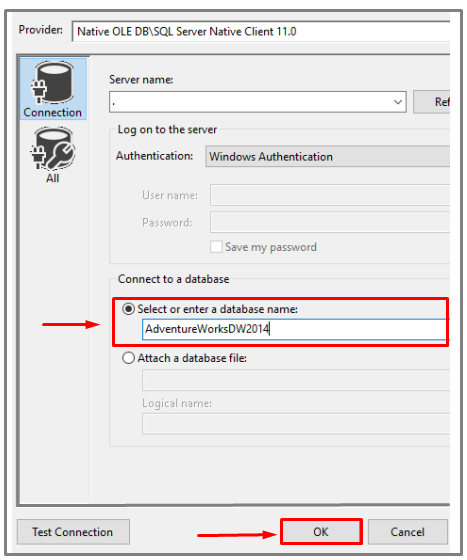
\includegraphics[width=8cm]{images/task1/img5}
    \end{center}	
Si todo está bien nos aparecerá la conexión creada en la sección de Data connections:
	\begin{center}
	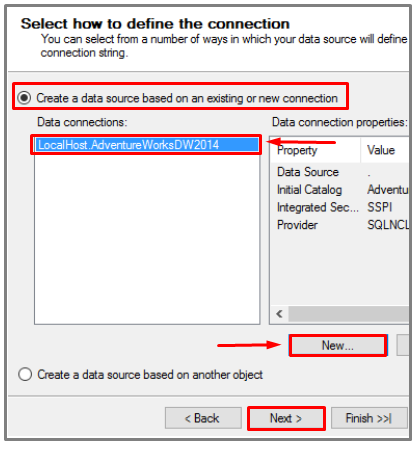
\includegraphics[width=8cm]{images/task1/img6}
    \end{center}	
En la ventana siguiente podemos definir las credenciales del Analysis Services y que utilizará para conectarse
al Data Source. En este caso utilizaremos las mismas credenciales del servicio. Para eso elegimos Use the
service account    
	\begin{center}
	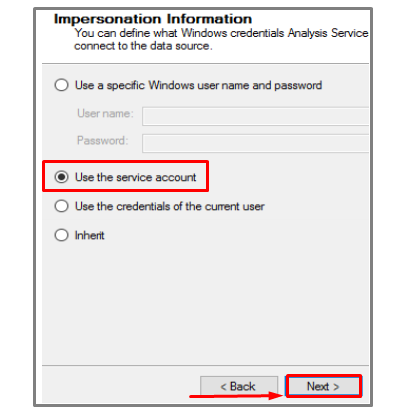
\includegraphics[width=8cm]{images/task1/img7}
    \end{center}	
Click en Next.
Colocamos un nombre para el Data Source y click en Finish:    
	\begin{center}
	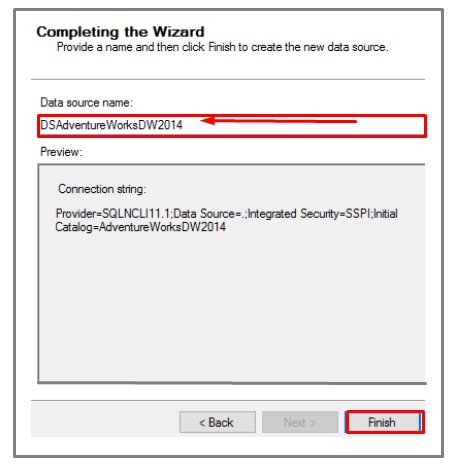
\includegraphics[width=8cm]{images/task1/img8}
    \end{center}	
   
\section{Creación de un Data Source View} 

En el Solution Explorer nos ubicamos en Data Sources View y click derecho, seleccionando la opción de
New Data Source View …
	\begin{center}
	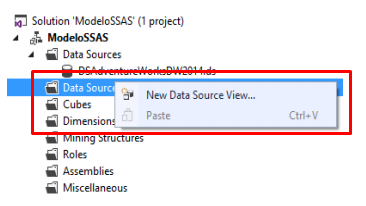
\includegraphics[width=8cm]{images/task2/img9}
	\end{center}	

Se nos abrirá una ventana de resumen. Click en Next:
\begin{center}
	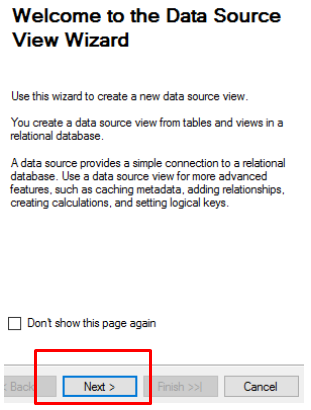
\includegraphics[width=8cm]{images/task2/img10}
\end{center}
Aquí nos aparecerán todos los Data Sources creados en la proyecto, en mi caso nos aparece el creado en
la sección 1. Click en Next:

\begin{center}
	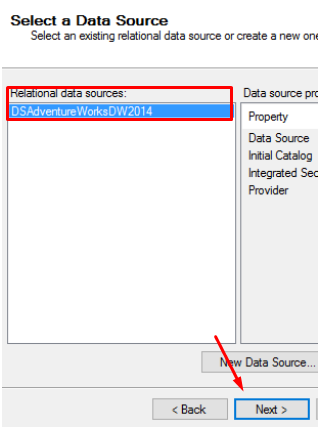
\includegraphics[width=8cm]{images/task2/img11}
\end{center}
Si bien es cierto hemos creado una conexión hacia Adventure Works DW, solo trabajaremos con algunas
tablas. Seleccionamos las tablas DimDate,DimProduct y FactInternetSales:
\begin{center}
	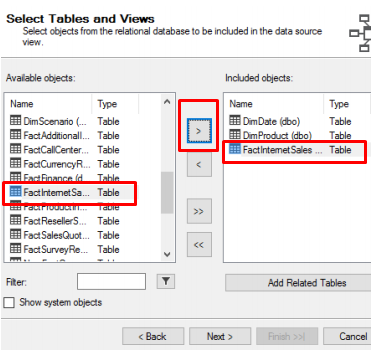
\includegraphics[width=8cm]{images/task2/img12}
\end{center}
Click en Next.
Colocamos un nombre el Data Source View creado y click en Finish:
\begin{center}
	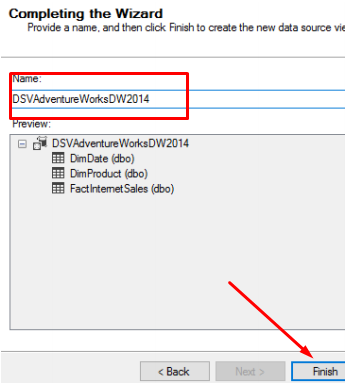
\includegraphics[width=8cm]{images/task2/img13}
\end{center}
Si todo va bien visualizaremos las tablas seleccionadas en el Data Source View:
\begin{center}
	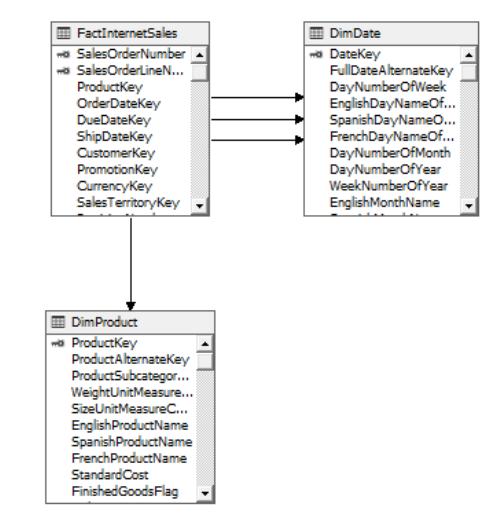
\includegraphics[width=8cm]{images/task2/img14}
\end{center}
\section{Creación de un Cubo}  

En el Solution Explorer nos ubicamos en Cubes y click derecho, seleccionando la opción de New Cube …
	\begin{center}
	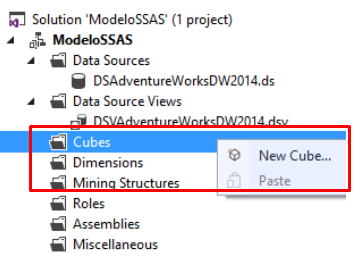
\includegraphics[width=8cm]{images/task3/img15}
	\end{center}	
Se nos abrirá una ventana de resumen. Click en Next:
	\begin{center}
	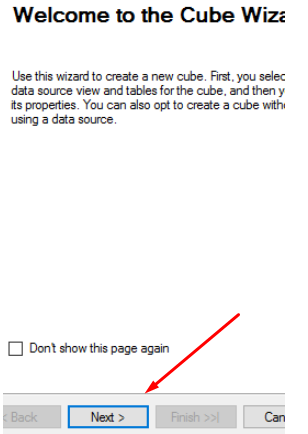
\includegraphics[width=8cm]{images/task3/img16}
	\end{center}	
Para la creación de un cubo tenemos varias opciones.
Use existing tables: Utilizar tablas del Data Source View.
Create an empty cube: Crear un cubo vacío.
Generate tables in the data source: Nos da la opción de crear tablas a partir de templates.
En este caso utilizaremos las tablas seleccionadas en el Data Source View creada en la sección 2:
	\begin{center}
	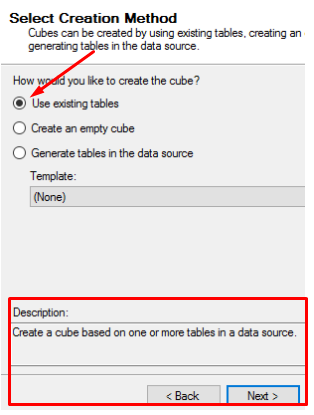
\includegraphics[width=8cm]{images/task3/img17}
	\end{center}	
Click en Next.
Aquí seleccionaremos la FactTable (Tablas de Hechos) , en este caso ubicamos FactInternetSales:
	\begin{center}
	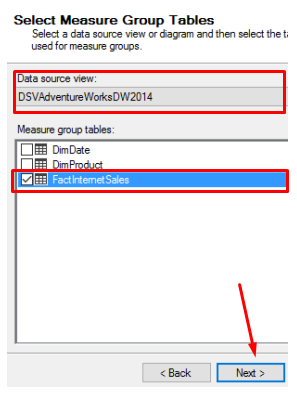
\includegraphics[width=8cm]{images/task3/img18}
	\end{center}	
Click en Next.
Automáticamente el Data Tools identificará todos los campos numéricos y los marcará como candidatos a
ser medidas. Podemos observar que inclusive marca los campos utilizados como Foregin Keys. En este
caso, seleccionamos solo Order Quantity y Sales Amount:
	\begin{center}
	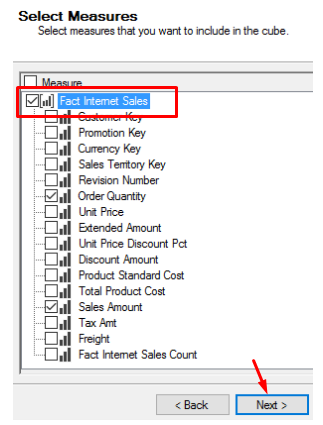
\includegraphics[width=8cm]{images/task3/img19}
	\end{center}	
Click en Next.
Aquí seleccionamos las dimensiones por las cuales será analizada la data. Inclusive el Data Tools te indica
que podría tomar la misma FactTable como Dimensión. Seleccionamos Dim Date y Dim Product:
	\begin{center}
	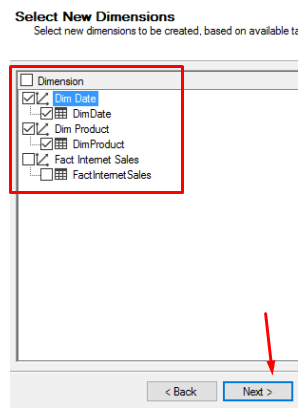
\includegraphics[width=8cm]{images/task3/img20}
	\end{center}	
Click en Next.
Colocamos un nombre el cubo:

	\begin{center}
	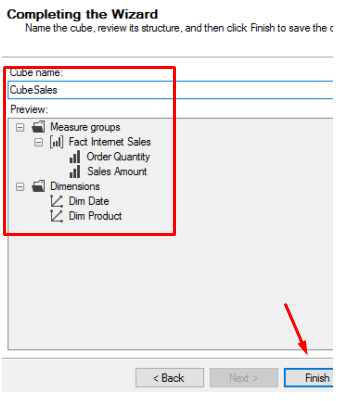
\includegraphics[width=8cm]{images/task3/img21}
	\end{center}	

Click en Finish
\section{Procesar Cubo} 
En el Solution Explorer nos ubicamos en el nuevo cubo creado CubeSales y click derecho, seleccionando la
opción de Process …

	\begin{center}
	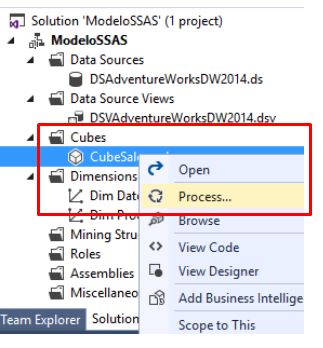
\includegraphics[width=8cm]{images/task4/img22}
	\end{center}	
	Click en Yes
	\begin{center}
	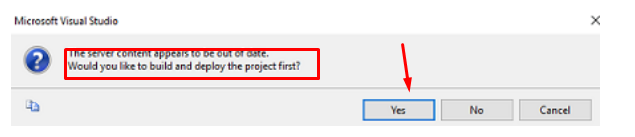
\includegraphics[width=8cm]{images/task4/img23}
	\end{center}	
En la nueva ventana seleccionamos la opción de Run…
	\begin{center}
	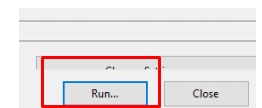
\includegraphics[width=8cm]{images/task4/img24}
	\end{center}	
Si todo va bien nos mostrará algo como lo siguiente:
	\begin{center}
	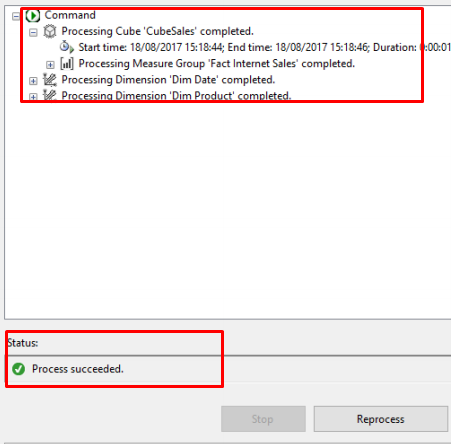
\includegraphics[width=8cm]{images/task4/img25}
	\end{center}	
Para verificar que nuestros datos se procesaron de forma correcta , en el cubo CubeSales nos dirigimos a la
pestaña de Browse:
	\begin{center}
	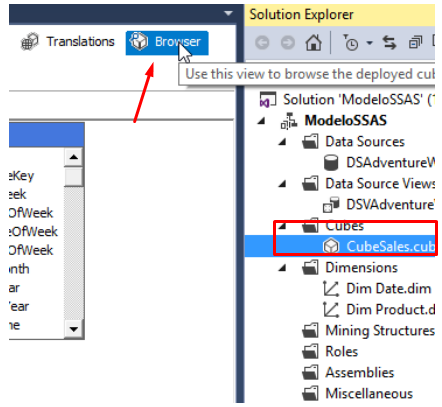
\includegraphics[width=8cm]{images/task4/img26}
	\end{center}	
En la pestaña de CubeSales, podemos tener un vistazo de las medidas y dimensiones. Arrastramos las
columnas de la Fact y la Dimensión Product obteniendo algo como:
	\begin{center}
	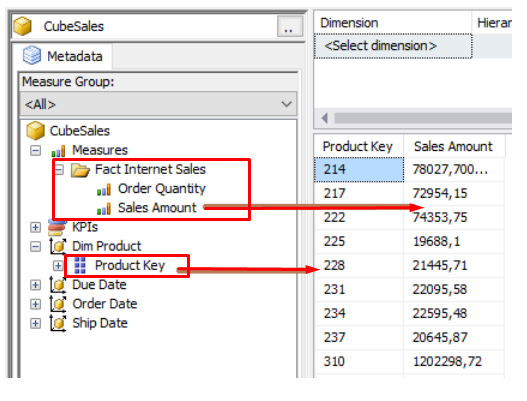
\includegraphics[width=8cm]{images/task4/img27}
	\end{center}	


\end{document}